\documentclass[a4paper,12pt]{article} 



%Добавляет возможность искать и копировать текст
\usepackage{cmap}

%Убирает пробел между названием таблицы/рисунка и самой таблицей/рисунком
\usepackage{caption}
\captionsetup[table]{skip= -0 cm}
\captionsetup[figure]{skip= -0 cm}

%Выравнивание названия таблиц по левому краю
%\usepackage[nooneline]{caption} 
%Размеры отступов 
\usepackage[left=20mm, top=20mm, right=20mm, bottom=20mm, footskip=10mm]{geometry}

%Рисунки
\usepackage{graphicx}
\usepackage{wrapfig} %обтекание элементов
\graphicspath{{graphs}{figures}}  % папки с картинками

%Русский язык в формулах
\usepackage{mathtext}

%  Русский язык
\usepackage[T2A]{fontenc}			
\usepackage[utf8]{inputenc}			
\usepackage[english,russian]{babel}	

%Готические буквы
\usepackage{amssymb}

% Математика
\usepackage{amsmath,amsfonts,amssymb,amsthm,mathtools} 
\usepackage{wasysym}

%Цветные подписи в таблице
\usepackage[table,xcdraw]{xcolor}

\usepackage{fancyhdr} % Колонтитулы
 	\pagestyle{fancy}
 	\renewcommand{\headrulewidth}{0.3mm}  % Толщина линейки, отчеркивающей верхний колонтитул
 	%\lfoot{Нижний левый}
 	%\rfoot{Нижний правый}
 	\rhead{Белостоцкий Артмемий, Б04-006}
 	%\chead{Верхний в центре}
 	\lhead{Лабораторная работа №4.1.2}
 	% \cfoot{Нижний в центре} % По умолчанию здесь номер страницы
 	
 	
\begin{document} 

%Титульник 
\begin{titlepage}
	\begin{center}
		\large 	МИНИСТЕРСТВО ОБРАЗОВАНИЯ И НАУКИ РОССИЙСКОЙ ФЕДЕРАЦИИ\\
				МОСКОВСКИЙ ФИЗИКО-ТЕХНИЧЕСКИЙ ИНСТИТУТ \\
				(НАЦИОНАЛЬНЫЙ ИССЛЕДОВАТЕЛЬСКИЙ ИНСТИТУТ)\\ 
				ФИЗТЕХ-ШКОЛА ЭЛЕКТРОНИКИ, ФОТОНИКИ \\
				И МОЛЕКУЛЯРНОЙ ФИЗИКИ \\
		
		
		\vspace{4.0 cm}
		Лабораторная работа № 4.1.2 \\ 
		\LARGE \textbf{Моделирование оптических приборов и определение их увеличения}
	\end{center}
	\vspace{3 cm} \large
	
	\begin{flushright}
		выполнил студент 2 курса \\
		{группы Б04-006}\\
		\textbf{Белостоцкий Артемий}\\
	\end{flushright}
	
	\vfill

	\begin{center}
	Долгопрудный, 2021 г.
	\end{center}
\end{titlepage}                                                                      


\section*{Цель работы}
Изучить модели зрительных труб (астрономической трубы Кеплера и земной трубы Галилея) и микроскопа, определить их увеличения.

\section*{В работе используются}

\begin{itemize}
\item оптическая скамья
\item набор линз
\item экран 
\item осветитель со шкалой
\item зрительная труба 
\item диафрагма 
\item линейка
\end{itemize}

\section*{Ход работы}

\subsubsection*{Определение фокусных расстояний линз}

\begin{wrapfigure}{r}{0.35\linewidth} 
	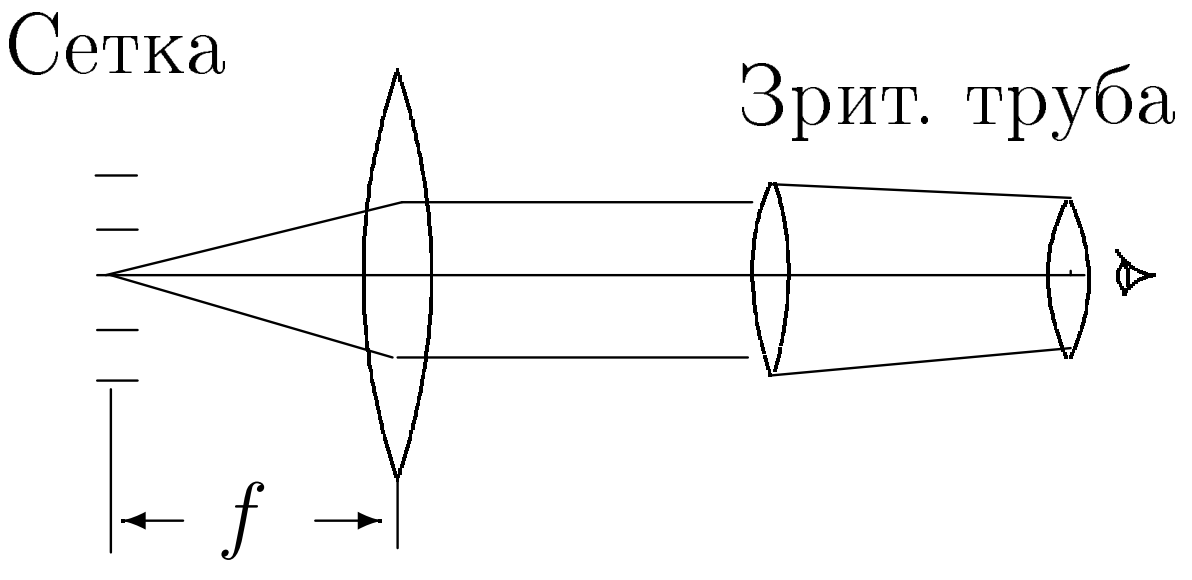
\includegraphics[width=\linewidth]{fig1}
	\caption{Определение фокусного расстояния собирающих линз}
	\label{collecting_lens}
\end{wrapfigure}
Центрируем оптическую систему. Настроим зрительную трубу на бесконечность. Установим собирающую линзу на на расстоянии от сетки примерно равном фокусному. На небольшом расстоянии от линзы закрепим трубу и отцентрируем по высоте.

Передвигая линзу вдоль скамьи, получим в окуляре зрительной трубы изображение миллиметровой сетки. При этом расстояние между сеткой и серединой линзы равно фокусному.

Повернем линзу другой стороной к источнику и повторим измерения фокусного расстояния. Занесем полученные данные в Таблицу 1.

\begin{table}[h]
\label{collecting_focuses}
	\begin{center}
	\caption{Значения фокусных расстояний для собирающих линз}
		\begin{tabular}{|c|c|c|}
		\hline
		\textbf{Линза} & \textbf{$f$, см} & \textbf{$f_{обр}$, см} \\ 		\hline
		№1             & 8,3            & 8,2                 \\ 	\hline
		№2             & 10,3           & 10,2                \\ \hline
		№3             & 19,5           & 19,5                \\ \hline
		№4             & 32             & 31                  \\ \hline
		\end{tabular}

	\end{center}
\end{table}

\newpage

\begin{wrapfigure}{l}{0.4\linewidth} 
	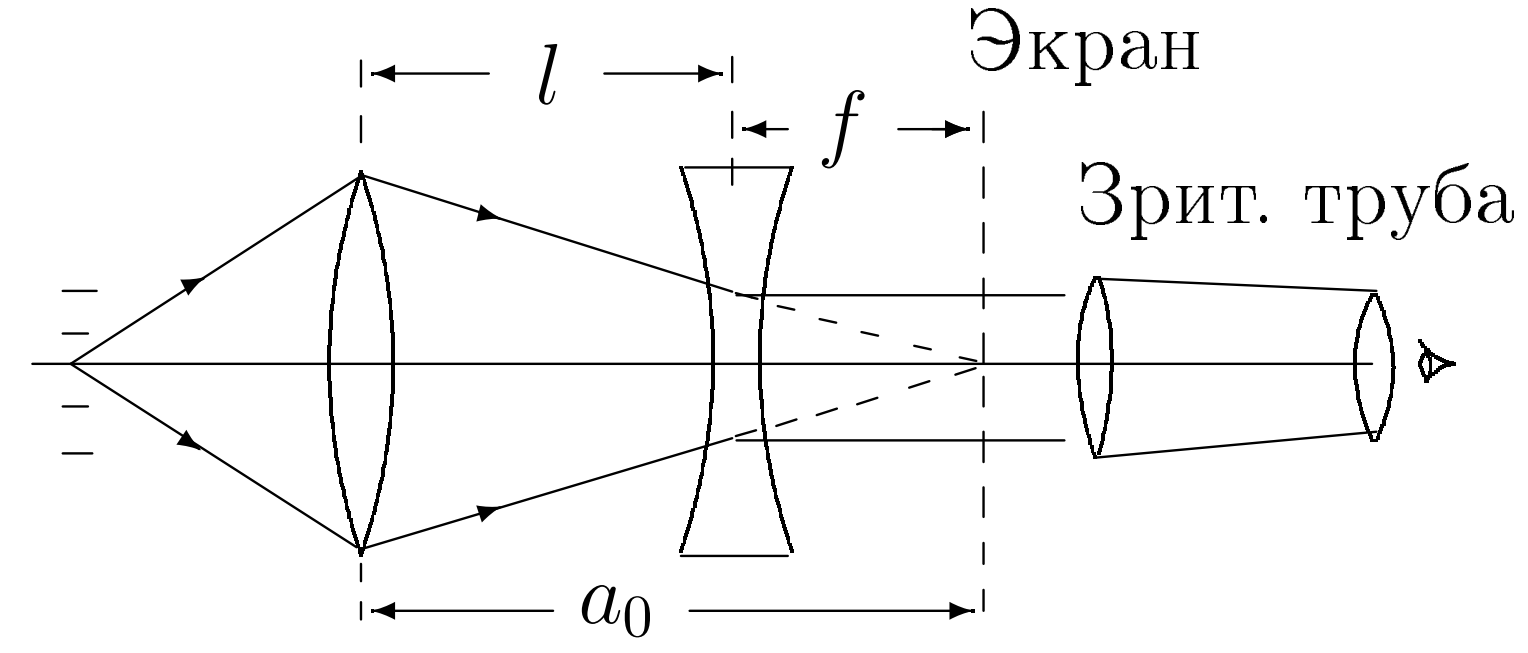
\includegraphics[width=\linewidth]{fig2}
	\caption{Определение фокусного расстояния рассеивающей линзы}
	\label{collecting_lens}
\end{wrapfigure}

Для определения фокусного расстояния тонкой рассеивающей линзы получим изображение сетки на экране при помощи короткофокусной собирающей линзы (причем $a_0 = 31 см$). Разместим за экраном трубу, настроенную на бесконечность, закрепим ее и уберем экран. 

Перемещая рассеивающую линзу, найдем в окуляре зрительной трубы резкое изображение сетки. Измерив расстояние между линзами $l$, рассчитаем фокусное расстояние рассеивающей линзы $f = l - a_0$. Перевернем рассеивающую линзы другой стороной к источнику и повторим измерения. Полученные данные занесем в Таблицу 2.

\begin{table}[h]
	\begin{center}
	\caption{Значения фокусных расстояний для рассеивающих линз}
	\begin{tabular}{|c|c|c|c|c|}
	\hline
	\textbf{Линза} & \textbf{$l$, см} & \textbf{$l_{обр}$, см} & \textbf{$f$, см} & 			\textbf{$f_{обр}$, см} \\ \hline
	№5    & 22    & 20,5       & 9              & 10,5                	\\ \hline
	\end{tabular}
	\end{center}
\end{table}

Сделаем вывод о тонкости линз. Так как для линз №1 - №3: $f - f_{обр} \sim \sigma_{f} = 0,1 \ см$ -- погрешность линейки, эти линзы можно считать тонкими.

\subsubsection*{Телескоп Кеплера}

\begin{wrapfigure}{r}{0.4\linewidth} 
	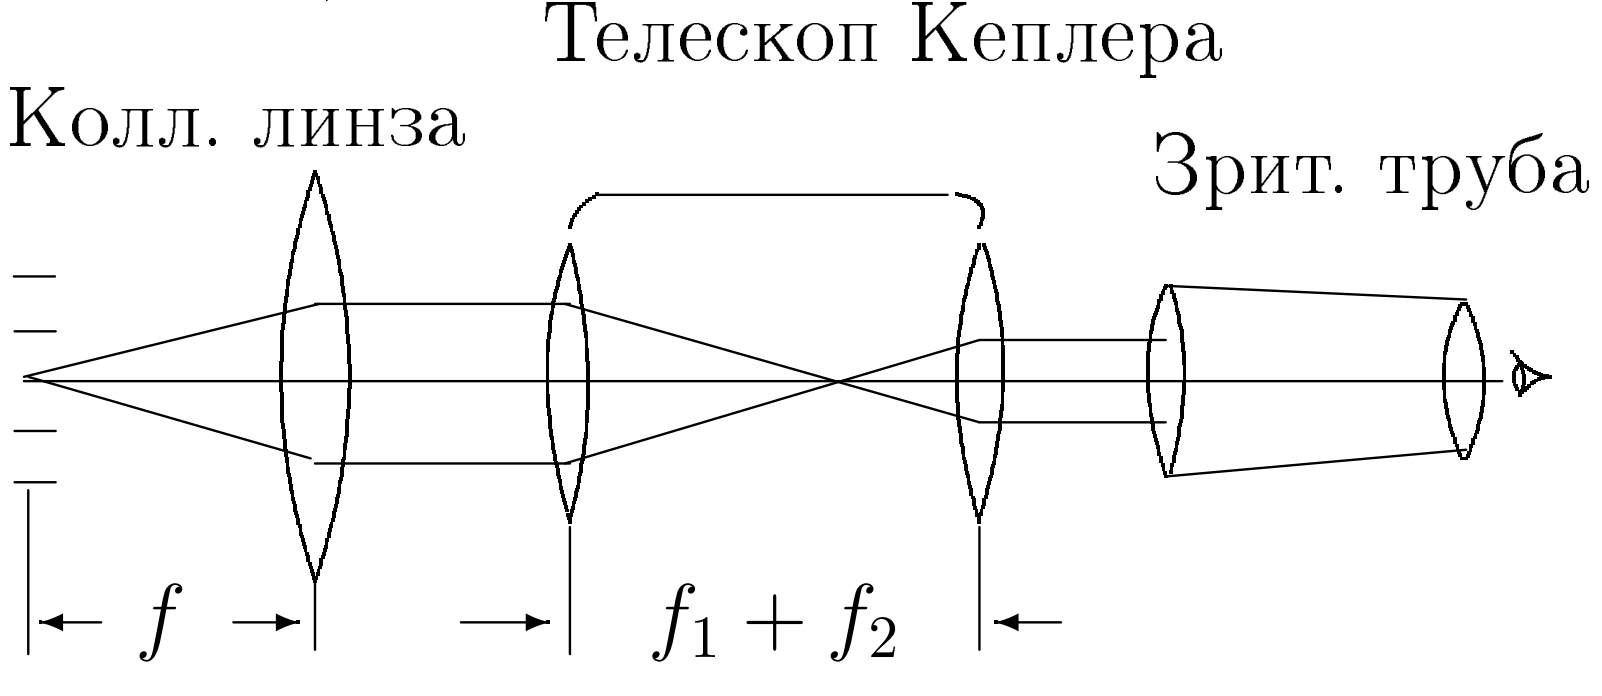
\includegraphics[width=\linewidth]{fig3}
	\caption{Модель телескопа}
	\label{Kepler}
\end{wrapfigure}

Соберем модель телескопа: линза с максимальным фокусным расстоянием -- объектив модели -- расположим вплотную к линзе коллиматора, окуляр -- на расстоянии, примерно равном сумме фокусных расстояний обеих линз телескопа.

Закрепим зрительную трубу за окуляром модели и отцентрируем световое пятно. Перемещая окуляр вдоль оптической скамьи получим изображение миллиметровой сетки в окуляре трубы.

Рассчитаем увеличение исследуемой модели телескопа по формуле:

$$
N_{T1} = \frac{f_1}{f_2} \approx 3,86 \pm  0,05
$$

, где $f_1 = 32 \ см; \ f_2 = 8,3 \ см $.

Определим размер изображения $h_1$ -- одного миллиметра шкалы осветителя в делениях окулярной шкалы зрительной трубы (без телескопа) и $h_2$ -- аналогичный размер с телескопом. Тогда:

$$
N_{T2} = \frac{h_2}{h_1} \approx 3,89 \pm 0,45
$$

, где $h_1 = 9 \ дел; \ h_2 = 35 \ дел$.

Погрешности рассчитывались по формулам:

$$
\sigma_{N_{T1}} =N_{T1} \sqrt{ \left(\frac{ \sigma_f}{f_1}\right)^2 + \left( \frac{\sigma_f}{f_2}\right)^2 }
$$
$$
\sigma_{N_{T2}} =N_{T2} \sqrt{ \left(\frac{ \sigma_h}{h_1}\right)^2 + \left( \frac{\sigma_h}{h_2}\right)^2 } , \sigma_h = 1 \ дел
$$

\newpage

\subsubsection*{Труба Галилея}

Вместо собирающей окулярной линзы поставим рассеивающую на расстоянии от объектива, равном разности фокусов объектива и окуляра. Дальнейшие измерение выполним аналогично телескопу Кеплера.

$$
N_{Г1} = \frac{f_1}{f_2} \approx 3,56 \pm  0,04
$$

, где $f_1 = 32 \ см; \ f_2 = 9 \ см $.


$$
N_{Г2} = \frac{h_2}{h_1} \approx 3,67 \pm 0,42
$$

, где $h_1 = 9 \ дел; \ h_2 = 33 \ дел$.


\subsubsection*{Модель микроскопа}

\begin{wrapfigure}{r}{0.361\linewidth} 
	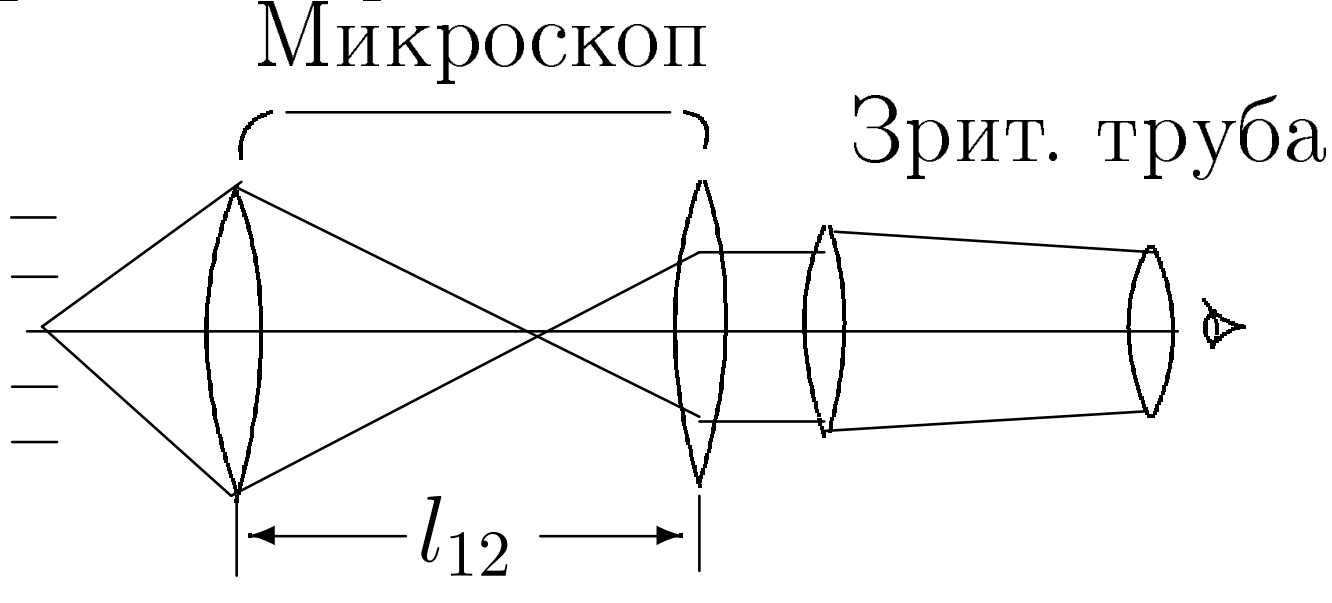
\includegraphics[width=\linewidth]{fig4}
	\caption{Модель микроскопа}
	\label{microscope}
\end{wrapfigure}

Отберем самые короткофокусные линзы ($f_1 = 8,3 \ см; f_2 = \ =10,3 \ см$), расположим объектив и окуляр на расстоянии $l_{12} = 35 \ см$ (подбираем так, чтобы увеличение было примерно равно 5) друг от друга. Сфокусируем модель микроскопа на сетке.

Получим изображение сетки на окуляре зрительной трубки. Измерим величину изображения $h_2$ миллиметрового деления предметной шкалы. Рассчитаем увеличение микроскопа двумя способами:

$$
N_{M1} = \frac{(l_{12}-f_1-f_2)L}{f_1 f_2} \approx 4,80
$$

$$
N_{M2} = \frac{h_2 L}{h_1 f_2} \approx 4,69 \pm 0,34
$$

, где L = 25 см, $h_1 = 16 \ дел; \ h_2 = 30 \ дел$

Погрешности рассчитывались по формулам:

$$
\sigma_{N_{M2}} = N_{M2} \sqrt{ \left(\frac{ \sigma_f}{f}\right)^2 + \left(\frac{ \sigma_f}{L}\right)^2 + \left(\frac{ \sigma_h}{h_1}\right)^2 + \left(\frac{ \sigma_h}{h_2}\right)^2 }
$$

\section*{Выводы}
1.В результате работы, несколькими способами были получены увеличения оптических приборов. \\
2.Для всех приборов увеличения, рассчитанные разными способами совпадают в пределах погрешности.


\end{document}
